%!TEX TS-program =  pdflatex 


\documentclass{amsart}
\usepackage{array}
\newcolumntype{P}[1]{>{\raggedright\let\newline\\\arraybackslash\hspace{0pt}}m{#1}}
\usepackage{graphicx,verbatim, amsmath, amssymb, amsthm, amsfonts, epsfig, amsxtra,ifthen,mathtools,epstopdf,caption,enumerate,hyperref,hhline,bbm,capt-of,longtable}	
\DeclareFontFamily{U}{mathx}{\hyphenchar\font45}
\DeclareFontShape{U}{mathx}{m}{n}{<-> mathx10}{}
\DeclareSymbolFont{mathx}{U}{mathx}{m}{n}
\DeclareMathAccent{\widebar}{0}{mathx}{"73}
\epstopdfsetup{suffix=}
\DeclareGraphicsExtensions{.ps}
\DeclareGraphicsRule{.ps}{pdf}{.pdf}{`ps2pdf -dEPSCrop -dNOSAFER #1 \noexpand\OutputFile}

\newtheorem{proposition}{Proposition}[section]
\newtheorem{theorem}[proposition]{Theorem}
\newtheorem{corollary}[proposition]{Corollary}
\newtheorem{lemma}[proposition]{Lemma}
\newtheorem{prop}[proposition]{Proposition}
\newtheorem{cor}[proposition]{Corollary}
\newtheorem{thm}[proposition]{Theorem}
\newtheorem{conj}[proposition]{Conjecture}
\newtheorem{phen}{Phenomenon} 

\renewcommand\thephen{\Roman{phen}}

\theoremstyle{definition}
\newtheorem{example}[proposition]{Example}
\newtheorem{definition}[proposition]{Definition}
\newtheorem{question}[proposition]{Question}

\theoremstyle{remark}
\newtheorem{remark}[proposition]{Remark}
\newtheorem{problem}[proposition]{Problem}

\numberwithin{equation}{section}
\usepackage[usenames]{color}

% commands for marginal notes below
% to make a marginal note, insert
% \margin{Your comment here.} in the text.
%  To sign the note:
% \margin[You]{Your comment here.}
% You can also label your comments and get a reference to the 
% number later, like:
% \margin[You]{Your comment here. \label{thefrivolouscomment}}
% Things may start to look ugly if you have more than 99 
%  marginal notes, but utility, not beauty is the intention here.
%  This uses the command \marginpar
%  defined, I think, in verbatim
%  The circled numbers will screw up the formatting slightly.

% Sometimes, if you terminate a run of LaTeX with "X" while using this macro, the next time you compile you will get the error "! File ended while scanning use of \@newl@bel.". The solution is to delete the .aux file (and fix whatever made you abort the run in the first place) and run LaTeX again.
% Another solution seems to be to terminate the new run with "q" and then run again.
\usepackage{color}

% to set color for comment numbers, use any of the 68 colors from 
% the color package in the command below
\newcommand{\margincolor}{red}      
\definecolor{darkgreen}{rgb}{0,0.7,0}
\newcommand{\marginauthorcolor}{darkgreen}      

% control the width of your comments
\addtolength{\marginparwidth}{8mm}

\newcounter{margincounter}
\setcounter{margincounter}{0}

\newcommand{\marginnum}{
\ifnum\value{margincounter}<10
\textcolor{\margincolor}{\begin{picture}(0,0)\put(2.2,2.4){\circle{9}}\end{picture}\footnotesize\arabic{margincounter}}
\else\ifnum\value{margincounter}<100
\textcolor{\margincolor}{\begin{picture}(0,0)\put(4.256,2.5){\circle{11}}\end{picture}\footnotesize\arabic{margincounter}}
\else
\textcolor{\margincolor}{\begin{picture}(0,0)\put(6.8,2.5){\circle{14}}\end{picture}\footnotesize\arabic{margincounter}}
\fi\fi
}

%\newcommand{\marginnum}{\textcolor{\margincolor}{\begin{picture}(0,0)\put(4.256,2.5){\circle{11}}\end{picture}\footnotesize\arabic{margincounter}}}


\newcommand{\margin}[2][]
{\!\!\refstepcounter{margincounter}\marginnum\marginpar{\textcolor{\margincolor}{\arabic{margincounter}.}\,\,\tiny #2\,\,\,\textcolor{\marginauthorcolor}{\small#1}}}
%  If you want to switch which margin you're using, do the command  \reversemarginpar before your marginal comment.
% To switch back, do \normalmarginpar
% (But I think it won't let you switch which margin you use in the middle of a paragraph of the main text.

%  to remove marginal notes, uncomment the following:
%  \renewcommand{\margin}[2][]{}
%  to remove just the circled numbers in the text, uncomment the following:
%  \renewcommand{\marginnum}{}
%  For final versions of a paper, it's probably best to remove all the \margin
%  commands.  Much to my annoyance, they mess up the typesetting.
\newcommand{\marginN}[1]{\margin[NR]{#1}}
\newcommand{\marginS}[1]{\margin[SV]{#1}}
\newcommand{\marginG}[1]{\margin[GM]{#1}}


% This is for setting off words we define in a separate typeface.
\newcommand{\newword}[1]{\textbf{\emph{#1}}}

\newcommand{\integers}{\mathbb Z}
\newcommand{\rationals}{\mathbb Q}
\newcommand{\naturals}{\mathbb N}
\newcommand{\reals}{\mathbb R}

\newcommand{\ep}{\varepsilon}
\newcommand{\thet}{\vartheta}
\newcommand{\col}{\mathbf{col}}
\newcommand{\id}{\operatorname{id}}
\newcommand{\cl}{\operatorname{cl}}
\newcommand{\cw}{\operatorname{cw}}
\newcommand{\ccw}{\operatorname{ccw}}
\newcommand{\sgn}{\operatorname{sgn}}
\newcommand{\vsgn}{\mathbf{sgn}}
\newcommand{\Seed}{\operatorname{Seed}}
\newcommand{\Sh}{{\mathcal Sh}}
\newcommand{\lcm}{\operatorname{lcm}}
\newcommand{\rank}{\operatorname{rank}}
\newcommand{\Int}{\operatorname{Int}}
\newcommand{\Fix}{\operatorname{Fix}}
\newcommand{\Stab}{\operatorname{Stab}}
\newcommand{\geom}{{\operatorname{geom}}}
\newcommand{\mon}{{\operatorname{mon}}}
\newcommand{\Ray}{{\operatorname{Ray}}}
\newcommand{\Ram}{{\operatorname{Ram}}}
\newcommand{\uf}{{\operatorname{uf}}}
\newcommand{\fr}{{\operatorname{fr}}}
\newcommand{\Geom}{{\operatorname{\textbf{Geom}}}}
\newcommand{\Cg}{\mbox{{\rm Cg}}}
\newcommand{\Con}{\mbox{{\rm Con}}}
\newcommand{\Irr}{\mbox{{\rm Irr}}}
\newcommand{\cov}{\mathrm{cov}}
\newcommand{\fs}{\mathrm{fs}}
\newcommand{\ufs}{\mathrm{ufs}}
\newcommand{\covers}{{\,\,\,\cdot\!\!\!\! >\,\,}}
\newcommand{\covered}{{\,\,<\!\!\!\!\cdot\,\,\,}}
\newcommand{\set}[1]{{\lbrace #1 \rbrace}}
\newcommand{\sett}[1]{{\bigl\lbrace #1 \bigr\rbrace}}
\newcommand{\settt}[1]{{\Bigl\lbrace #1 \Bigr\rbrace}}
\newcommand{\setttt}[1]{{\biggl\lbrace #1 \biggr\rbrace}}
\newcommand{\settttt}[1]{{\Biggl\lbrace #1 \Biggr\rbrace}}
\newcommand{\pidown}{\pi_\downarrow}
\newcommand{\piup}{\pi^\uparrow}
\newcommand{\br}[1]{{\langle #1 \rangle}}
\newcommand{\A}{{\mathcal A}}
\newcommand{\EL}{{\mathcal L}}
\newcommand{\F}{{\mathcal F}}
\newcommand{\D}{{\mathfrak D}}
\newcommand{\N}{{\mathcal N}}
\newcommand{\p}{{\mathfrak p}}
\newcommand{\X}{{\mathcal X}}
\newcommand{\W}{{\mathcal W}}
\newcommand{\join}{\vee}
\newcommand{\meet}{\wedge}
\renewcommand{\Join}{\bigvee}
\newcommand{\Meet}{\bigwedge}
\newcommand{\bigmeet}{\Meet}
\newcommand{\bigjoin}{\Join}
\newcommand{\leftq}[2]{\!\!\phantom{.}^{#1} {#2}}
\newcommand{\closeleftq}[2]{\!\!\phantom{.}^{#1}\! {#2}}
\newcommand{\Pge}{{\Phi_{\ge -1}}}
\newcommand{\cm}{\parallel}
%\newcommand{\ck}{^\vee}
%\newcommand{\ck}{^{\scalebox{0.5}[0.5]{$\vee$}}}
\newcommand{\ck}{\spcheck}
\newcommand{\letw}{\le_{\mathrm{tw}}}
\newcommand{\Alg}{\mathrm{Alg}}
\newcommand{\toname}[1]{\stackrel{#1}{\longrightarrow}}
\newcommand{\dashname}[1]{\stackrel{#1}{\mbox{---\!---}}}
\newcommand{\st}{^\mathrm{st}}
\renewcommand{\th}{^\text{th}}
\newcommand{\nd}{^\text{nd}}
\newcommand{\rd}{^\text{rd}}
\newcommand{\0}{{\mathbf{0}}}
\newcommand{\Vol}{\mathrm{Vol}}
\newcommand{\lleq}{\le\!\!\!\le}
\newcommand{\notlleq}{\le\!\!\!\!\not\,\le}
\newcommand{\ggeq}{\ge\!\!\!\ge}
\newcommand{\FF}{\mathcal{F}}
\newcommand{\ZZ}{\mathbb{Z}}
\newcommand{\QQ}{\mathbb{Q}}
\newcommand{\RR}{\mathbb{R}}
\newcommand{\CC}{\mathbb{C}}
\newcommand{\PP}{\mathbb{P}}
\newcommand{\GL}{\mathrm{GL}}
\newcommand{\Tits}{\mathrm{Tits}}
\newcommand{\Cone}{\mathrm{Cone}}
\newcommand{\Star}{\mathrm{Star}}
\newcommand{\Lin}{\mathrm{Lin}}
\newcommand{\Ker}{\mathrm{Ker}}
\newcommand{\Proj}{\mathrm{Proj}}
\newcommand{\relint}{\mathrm{relint}}
\newcommand{\Clust}{\mathrm{Clust}}
\newcommand{\into}{\hookrightarrow}
\newcommand{\equivalent}{\Longleftrightarrow}
\newcommand{\onto}{\twoheadrightarrow}
\newcommand{\isomorph}{\cong}
\newcommand{\diag}{\mathrm{diag}}
\newcommand{\Asym}{A_{\mathrm{sym}}}
\newcommand{\Cox}{\mathrm{Cox}}
\newcommand{\Des}{\mathrm{Des}}
\DeclareMathOperator{\Span}{Span}
\DeclareMathOperator{\supp}{supp}
\DeclareMathOperator{\inv}{inv}
\newcommand{\odd}{\mathrm{odd}}
\newcommand{\g}{\mathbf{g}}
\newcommand{\s}{\mathbf{s}}
\newcommand{\m}{\mathbf{m}}
\renewcommand{\c}{\mathbf{c}}
\renewcommand{\b}{\mathbf{b}}
\renewcommand{\k}{\mathbbm{k}}
\newcommand{\ks}{\mathbf{k}}
\renewcommand{\a}{\mathbf{a}}
\newcommand{\e}{\mathbf{e}}
\newcommand{\x}{\mathbf{x}}
\newcommand{\y}{\mathbf{y}}
\newcommand{\z}{\mathbf{z}}
\renewcommand{\t}{\mathbf{t}}
\renewcommand{\v}{\mathbf{v}}
\renewcommand{\u}{\mathbf{u}}
\newcommand{\w}{\mathbf{w}}
\newcommand{\tB}{\tilde{B}}
\newcommand{\T}{\mathbb{T}}
\newcommand{\ZP}{\mathbb{ZP}}
\newcommand{\C}{\mathcal{C}}
\newcommand{\B}{\mathcal{B}}
\newcommand{\M}{\mathbf{M}}
\newcommand{\R}{\mathcal{R}}
\renewcommand{\L}{\mathbf{L}}
\newcommand{\V}{\mathcal{V}}
\newcommand{\U}{\mathcal{U}}
\renewcommand{\O}{\mathcal{O}}
\renewcommand{\H}{\mathcal{H}}
\renewcommand{\P}{\mathbb{P}}
\newcommand{\K}{\mathbb{K}}
\newcommand{\Rel}{\operatorname{Rel}}
\newcommand{\Trop}{\operatorname{Trop}}
\newcommand{\Supp}{\operatorname{Supp}}
\newcommand{\pr}{{\operatorname{pr}}}
\newcommand{\bB}{\widebar{B}}
\renewcommand{\S}{\mathbf{S}}
\newcommand{\Var}{\operatorname{Var}}
\newcommand{\Hom}{\operatorname{Hom}}
\newcommand{\Scat}{\operatorname{Scat}}
\newcommand{\Fan}{\operatorname{Fan}}
\newcommand{\ScatFan}{\operatorname{ScatFan}}
\newcommand{\ClusFan}{\operatorname{ClusFan}}
\newcommand{\CambScat}{\operatorname{CambScat}}
\newcommand{\Nar}{\operatorname{Nar}}
\newcommand{\can}{\operatorname{can}}
\newcommand{\re}{\mathrm{re}}
\newcommand{\im}{\mathrm{im}}
%\newcommand{\init}{\mathrm{in}}
\renewcommand{\d}{{\mathfrak d}}
%\newcommand{\f}{{\mathfrak f}}
\newcommand{\seg}[1]{\overline{#1}}
\newcommand{\hy}{\hat{y}}
\newcommand{\notch}{^{\scalebox{0.6}{\raisebox{-3pt}{$\mathrel \blacktriangleright \joinrel \mathrel \blacktriangleleft$}}}}

\newcommand{\fakesubsec}[1]{\medskip\noindent\textbf{#1.}}  %unnumbered

%%%%%
%Greg's preamble stuff

\usepackage{tikz}
\usetikzlibrary{arrows,decorations.pathmorphing,decorations.markings,backgrounds,positioning,fit}
\tikzstyle{dot} = [fill=black!25,inner sep=0.5mm,circle,draw,minimum size=1mm]
\tikzstyle{marked}=[inner sep=0.5mm,circle,draw=blue!75!black,fill=blue!50]
\tikzstyle{lamination}=[green!75!black]
\tikzstyle{barricade}=[line width=4pt,decorate,decoration={markings,mark=between positions 0 and 1 step 6pt
	with { 
		\fill[yellow] (-2pt,-1pt) -- (1pt,-1pt) -- (2pt,1pt) -- (-1pt,1pt) -- (-2pt,-1pt);
		\fill[black] (1pt,-1pt) -- (4pt,-1pt) -- (5pt,1pt) -- (2pt,1pt) -- (1pt,-1pt);
	}}
]
\tikzstyle{barricade vertex}=[inner sep=0.6mm,thick,circle,draw=black,fill=yellow]

\newenvironment{ex}{\refstepcounter{proposition}\begin{proof}[Example \emph{\thethm}]\renewcommand*{\qedsymbol}{\(\blacksquare\)}}{\end{proof}}
\newenvironment{rem}{\refstepcounter{proposition}\begin{proof}[Remark \emph{\thethm}]\renewcommand*{\qedsymbol}{\(\blacksquare\)}}{\end{proof}}

%\Greg's preamble stuff
%%%%%

\title{Scattering diagrams for surfaces}
\author{Greg Muller, Nathan Reading, and Shira Viel}
%\date{}                                           % Activate to display a given date or no date
\thanks{Nathan Reading was partially supported by the National Science Foundation under Grant Number DMS-1500949.}
%\subjclass[2010]{13F60, 14N35, 52C99+ surfaces?}


\begin{document}

%\begin{abstract}
%\end{abstract}
%\maketitle
%
%%\vspace{-15pt}
%
%\setcounter{tocdepth}{2}
%\tableofcontents
%

\section{Introduction}\label{intro sec}  

%\marginN{Of course, it's not time to write this yet, but I'm recording some decisions explicitly, so that we can follow through with them (and mention them explicitly in the paper) or change them.}



\section{Triangulated marked surfaces}\label{surface sec}
In this section, we quote background material on the triangulated marked surfaces model from \cite{cats1,cats2}, with some modifications as in \cite{unisurface}.


\begin{definition}[\emph{Marked surface}]\label{S M def}
A \newword{marked surface} is a pair $(\S,\M)$ such that $\S$ is a compact, connected, oriented surface whose boundary is a (possibly empty) union of disjoint circles and $\M$ is a nonempty, finite collection of points in $\S$ called \newword{marked points}.
The circles forming the boundary of $\S$ are called \newword{boundary components}, and we require that there is at least one marked point in each boundary component.
Marked points that lie in the interior of $\S$ are called \newword{punctures}.
A \newword{boundary segment} is a curve contained in the boundary of $\S$ whose endpoints are in $\M$, with no points of $\M$ in the interior of the curve.
If $\S$ is a disk with three or fewer marked points on its boundary, then $(\S,\M)$ must have at least one puncture.
If $\S$ is a disk with only one marked point on its boundary (a monogon), then it must have at least two punctures.
If $\S$ is a sphere, then it must have at least $4$ punctures.  
(It is harmless, and sometimes convenient as in \cite{dominance}, to allow $\S$ to be disconnected and/or to allow once-punctured monogons, but there is no need here.)
\end{definition}

\begin{definition}[\emph{Arcs and triangulations}]\label{tri def}
An \newword{arc} in $(\S,\M)$ is a curve in $\S$ with endpoints in $\M$.
The arc may not intersect itself and, except at its endpoints, must be contained in the interior of $\S\setminus\M$.
The arc may not bound an unpunctured monogon and may not define, together with a boundary segment connecting the endpoints, an unpunctured digon.
Throughout, we consider arcs up to isotopy equivalence.

Two arcs are \newword{compatible} is there is an isotopy representative of each such that the representatives do not intersect, except possibly at their endpoints.
A \newword{triangulation} $T$ is a maximal collection of distinct pairwise compatible arcs.
The connected components of $\S\setminus\cup T$ are \newword{triangles}, which have one, two or three distinct vertices (in $\M$) and two or three distinct sides (in $T$).
A triangle is called \newword{self-folded} if it has only two distinct sides.
The arc that defines two different sides of the triangle is the \newword{fold edge}.
\marginN{for now, I don't think we need to discuss flips}
\end{definition}

\begin{definition}[\emph{Signed adjacency matrix}]\label{B(T) def}
Given a triangulation $T$, we define a skew-symmetric integer matrix $B(T)=[b_{\alpha\beta}]_{\alpha,\beta\in T}$.
To do so we define a map $\pi_T$ on the arcs of $T$ sending the fold edge of each self-folded triangle in $T$ to the other edge of the same triangle, and fixing all other arcs.
We define $b_{\alpha\beta}$ to be the sum $\sum_\Delta b^\Delta_{\alpha\beta}$, over all \emph{non-self-folded} triangles $\Delta$ of $T$, where 
\[b^\Delta_{\alpha\beta}=
\begin{cases} 
\,\,\,\,\,1&\text{if $\Delta$ has sides $\pi_T(\alpha)$ and $\pi_T(\beta)$ such that $\pi_T(\alpha)$} \\[-2pt]&\quad\text{is immediately followed by $\pi_T(\beta)$ in \emph{clockwise} order.}\\[3pt]
\,-1&\text{if $\Delta$ has sides $\pi_T(\alpha)$ and $\pi_T(\beta)$ such that $\pi_T(\alpha)$} \\[-2pt]&\quad\text{is immediately followed by $\pi_T(\beta)$ in \emph{counterclockwise} order.}\\[3pt]
\,\,\,\,\,0&\text{otherwise.}
\end{cases}
\]
\end{definition}

\begin{definition}[\emph{Allowable curve}]\label{allowable def}
An \newword{allowable curve} in $(\S,\M)$ is  
\begin{itemize}
\item a closed curve,
\item a curve whose two endpoints are unmarked boundary points,
\item a curve having one endpoint an unmarked boundary point, with the other end spiraling (clockwise or counterclockwise) into a puncture, or
\item a curve spiraling into (not necessarily distinct) punctures at both ends,
\end{itemize}
that
\begin{itemize}
\item has no self-intersections,
\item is not contractible in $\S\setminus\M$,
\item is not a closed curve contractible in $\S\setminus\M$ to a puncture,
\item is not contractible (by an isotopy fixing its endpoints) to a portion of the boundary containing zero or one marked points,
\item does not have both endpoints on the same boundary segment and, together with the portion of the boundary between its endpoints, cut out a once-punctured disk, and 
\item does not spiral at both ends into the same marked point and cut out an unpunctured or once-punctured disk.
\end{itemize}
\end{definition}

\begin{definition}[\emph{Quasi-laminations}]\label{quasilam def}
Two allowable curves are \newword{compatible} if 
\begin{itemize}
\item
they are nonintersecting, or 
\item they are identical except that, at exactly one end of the curve, they spiral opposite directions into the same marked point.
\end{itemize}
A \newword{(rational) quasi-lamination} $L$ in $(\S,\M)$ is a collection of pairwise compatible allowable curves in $\S$, distinct up to isotopy, with each curve $\lambda\in L$ carrying a positive rational weight $w_\lambda$.
A \newword{multi-lamination} is a finite collection $\L$ of laminations.
\end{definition}

\begin{definition}[\emph{Honest embedding}]\label{honest def}  \marginN{Unless I'm mistaken, this condition on an allowable curve is exactly the condition of minimizing the number of intersections with the arcs of $T$.  This way of saying it seems so much more clear to me.}
An embedding of a curve or circle in $\S\setminus\M$ is \newword{honest} \marginN{I like this term, but am not married to it.  If you hate it we can change it.}
if each intersection of the embedded curve with an arc of $T$ is transverse, and if the embedded curve never crosses an arc of $T$ and then crosses the same arc again \emph{in the opposite direction} without crossing a different arc of $T$ in between.
(The caveat about opposite directions is present in order to allow honest embeddings of allowable curves with spirals.
An allowable curve that spirals into the puncture in a self-folded triangle crosses the fold edge of the triangle infinitely many times in succession, but can be embedded honestly, because these crossings can be all in the same direction.)

We also extend the definition to curves that are disjoint from $\M$ except for having an endpoint at the puncture inside a self-folded triangle.
To be honest, these must pass from the puncture to the interior of the self-folded triangle and be honest in the above sense elsewhere.
\end{definition}

\begin{remark}\label{honest curve}
An honestly embedded allowable curve determines a sequence of arcs of $T$ (infinite if the curve spirals at one end or indexed by $\integers$ if it spirals at both ends).
The sequence is the same (up to reversing) for every honest embedding, and the allowable curve is uniquely determined by the sequence.
\end{remark}


\begin{definition}[\emph{Shear coordinates}]\label{shear def}
Given a quasi-lamination $L$, a triangulation $T$, and an arc $\gamma\in T$,  we define the \newword{shear coordinate} $b_\gamma(T,L)$ of $L$ at $\gamma$ (with respect to $T$).
This is $b_\gamma(T,L)=\sum_{\lambda\in L}w_\lambda b_\gamma(T,\lambda)$, a weighted sum over curves $\lambda$ in $L$ of quantities $b_\gamma(T,\lambda)$ that we now define.
First, if $\gamma$ is \emph{not} the fold edge of a self-folded triangle of $T$, then it is contained in a quadrilateral.
(Possibly, the edges of this quadrilateral are fewer than four distinct arcs of $T$.)
We choose an honest isotopy representative of $\lambda$ (in the sense of Definition~\ref{honest def}) and we reuse the symbol $\lambda$ for the representative.
Each intersection of $\lambda$ with $\gamma$ contributes $-1$, $0$, or $1$ to $b_\gamma(T,\lambda)$.
The contribution is $0$ unless $\lambda$ intersects the triangles containing $\gamma$ in one of the ways shown in Figure~\ref{shear fig}, in which case the contribution is $1$ or $-1$ as shown.
(In the figure, $\gamma$ is the diagonal of the quadrilateral shown, and $\lambda$ is a vertical or horizontal dashed line.)
\begin{figure}[ht]
\raisebox{42 pt}{$+1$}\,\,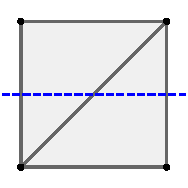
\includegraphics{shearplus}\qquad\qquad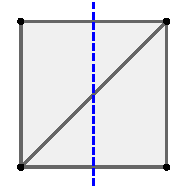
\includegraphics{shearminus}\,\,\raisebox{42 pt}{$-1$}
\caption{Computing shear coordinates}
\label{shear fig}
\end{figure}
If $\gamma$ \emph{is} the fold edge of a self-folded triangle of $T$, then $\gamma$ is inside a once-punctured monogon in $T$.
Let $p$ be punctured in that monogon, let $\gamma'$ be the other edge of that self-folded triangle, and let $\lambda'$ be the allowable curve obtained from $\lambda$ by reversing the direction of all spirals (if any) at  $p$.
Then define $b_\gamma(T,\lambda)$ to be $b_{\gamma'}(T,\lambda')$.
\end{definition}

\marginN{commented out here:  the theorem on laminations in bijection with rational vectors.  May want to quote this later when we set up the vector spaces, or maybe even later when we need it.}
%\begin{theorem}\label{q-lam bij}
%Fix a tagged triangulation $T$.
%Then the map $L\mapsto\b(T,L)$ is a bijection between integral (resp. rational) quasi-laminations and $\integers^n$ (resp.~$\rationals^n$).
%\end{theorem}


\marginN{commented out here is the definition of $\kappa$.  We will probably need it.}
%Given a tagged arc $\alpha$ in $(\S,\M)$, we define (up to isotopy) a curve $\kappa(\alpha)$.
%The curve $\kappa(\alpha)$ coincides with $\alpha$ except within a small ball around the endpoints of $\alpha$.
%Within each ball around an endpoint $p$, the behavior of $\kappa(\alpha)$ is as follows:
%If $p$ is on a boundary component, then $\kappa(\alpha)$ ends at a point $x$ on the same boundary component such the path along the boundary from $p$ to $x$, keeping $\S$ on the left, does not leave the small ball.
%If $p$ is a puncture, then $\kappa(\alpha)$ spirals into $p$, clockwise if $\alpha$ is tagged plain at $p$ and counterclockwise if $\alpha$ is tagged notched at $p$.
%The map $\kappa$ is similar to the map considered in \cite[Definition~17.2]{cats2}, but with the opposite orientation throughout.
%

\begin{remark}\label{comparison to cats1-2}
In \cite{cats1,cats2}, the interior of $\S\setminus\M$ is given the structure of Riemann surface, but the metric structure is not needed here.  \marginN{as far as I know now}
What we are calling triangles and triangulations are called ideal triangles and ideal triangulations in \cite{cats1,cats2} because their vertices are at infinity in the Riemannian metric.
In some papers, the term ``ideal triangulation'' is used to distinguish triangulations from ``tagged triangulations,'' which we will not need here.  \marginN{I think}
(Every tagged triangulation also has a signed adjacency matrix, but the definition is such that in every case, there is an ordinary triangulation with the same signed adjacency matrix \cite[Definition~9.18]{cats1}.)
The notion of a quasi-lamination is a slight variation (from \cite{unisurface}) on the laminations occurring in \cite{cats2}.
The point of the variation is that non-closed allowable curves correspond to tagged arcs.
\end{remark}

\section{Scattering diagrams}\label{scat sec}
The goal of this paper is to construct the cluster scattering diagram associated to a triangulated marked surface.
In this section, we review the background on scattering diagrams, but specifically in the context of a triangulated surface.
We have largely followed \cite{GHK,GHKK}, with some small changes, following~\cite{scatfan}.

In what follows, we fix a marked surface $(\S,\M)$, a \marginN{ordinary, here.  Can we get by entirely without tagged triangulations?  Would be nice.}
triangulation $T$ and a multi-lamination $\L$. 
The signed adjacency matrix $B(T)$ is in particular an exchange matrix.
(In general, an \newword{exchange matrix} is a skew-symmetrizable integer matrix.
The matrix $B(T)$ is more special:  It is skew-symmetric.)

The initial data defining a cluster scattering diagram amounts to an \newword{extended exchange matrix}.
There are two different conventions in the cluster algebras literature on extending an exchange matrix.
Here, we follow \cite{GHKK} in extending exchange matrices by adding columns of integer vectors.
(Switching from our \emph{wide} extended exchange matrices to the \emph{tall} extended exchange matrices of \cite{ca4} amounts to  transposing (or equivalently in the skew-symmetric case, negating) the exchange matrix.)

\begin{definition}[\emph{Extended exchange matrix for $T$ and $\L$}]\label{tB(T,L) def}
The extended exchange matrix $\tB(T,L)$ defined by $(\S,\M)$, $T$, and $\L$ has rows indexed by $T$ and columns indexed by $T\cup\L$.
Its entries $b_{\alpha\beta}$ for $\alpha,\beta\in T$ are the entries of the signed adjacency matrix $B(T)$ defined in Definition~\ref{B(T) def} and its entry $b_{\alpha L}$ for $\alpha\in T$ and $L\in\L$ is $b_\alpha(T,L)$ as in Definition~\ref{shear def}.
\end{definition}

Starting with $T$ and $\L$, we define the following objects.
(The extended exchange matrix $B(T,\L)$ appears as the bilinear form $\set{\,\cdot\,,\,\cdot\,}$.
\marginN{I've rethought a few of the ideas that were in the table before.  (Feel free to disagree.)  The main change is that I set up the dual lattice and vector space in terms of formal duals of the arcs in $T$ instead of as laminations.  We will still use laminations, of course, but I think this is cleaner.  Not sure if I like the table approach, but maybe it's not so bad, especially since the table got shorter. }



\renewcommand*{\arraystretch}{1.4}
\setlength{\doublerulesep}{0pt}
\begin{longtable}{P{88.5pt}|P{248pt}}
\caption{Initial data and preliminary definitions for scattering diagrams from surfaces}\label{init data}\\
Notation&Description/requirements\\\hline\hline\hline
\endfirsthead
\caption{(continued)}\\
Notation&Description/requirements\\\hline\hline\hline
\endhead
%Notation&Description/requirements\\\hline\hline\hline
%\endfirsthead
%\endhead
%\caption{Initial data and preliminary definitions for scattering diagrams}\label{init data}\\
%\endfoot
%\caption{(continued)}\\
%\endlastfoot
$N=N_\uf\oplus N_\fr$\linebreak %\hspace*{40pt} 
(a lattice) &
$\begin{aligned}N_\uf&=\textstyle\sett{\sum_{\gamma\in T}c_\gamma\gamma:\text{ each }c_\gamma\in\integers} \text{ (formal sums)}\\\
N_\fr&=\textstyle\sett{\sum_{L\in\L}c_LL:\text{ each }c_\gamma\in\integers}\end{aligned}$
\\\hline
$\begin{aligned}M&=\Hom(N,\integers)\\&=M_\uf\oplus M_\fr\end{aligned}$\linebreak %\hspace*{40pt} 
(dual lattice) 
&
$\begin{aligned}M_\uf&=\textstyle\sett{\sum_{\gamma\in T}c_\gamma\gamma^*:\text{ each }c_\gamma\in\integers}\\
M_\fr&=\textstyle\sett{\sum_{L\in\L}c_LL^*:\text{ each }c_\gamma\in\integers}\end{aligned}$\linebreak
for dual vectors $\gamma^*$ for $\gamma\in T$ and $L^*$ for $L\in\L$
\\\hline
$V=N_\uf\otimes_\integers\reals$&$V=\sett{\sum_{\gamma\in T}c_\gamma\gamma:\text{ each }c_\gamma\in\reals}$ \\\hline
$V^*=M_\uf\otimes_\integers\reals$\linebreak
(dual vector space)&
$V=\sett{\sum_{\gamma\in T}c_\gamma\gamma^*:\text{ each }c_\gamma\in\reals}$
\\\hline
$\br{\,\cdot\,,\,\cdot\,}:V^*\times V\to\reals$\linebreak
$\br{\,\cdot\,,\,\cdot\,}:M\times N\to\rationals$\linebreak
(the usual pairing)& 
$\br{\alpha^*,\gamma}=\delta_{\alpha\gamma}$ (Kronecker delta) for $\alpha,\gamma\in T$\linebreak
$\br{L^*,M}=\delta_{LM}$ (Kronecker delta) for $L,M\in\L$\linebreak
$\br{\alpha^*,L}=\br{L^*,\alpha}=0$ for $\alpha\in T$ and $L\in\L$
\\\hline
$\set{\,\cdot\,,\,\cdot\,}:N\times N\to\integers$\linebreak
(bilinear form)&$\set{\alpha,\gamma}=b_{\alpha_\gamma}$ (entry of $B(T)$) for $\alpha,\gamma\in T$\linebreak
$\set{\alpha,L}=b_\alpha(T,L)$ (shear coordinate) for $\alpha\in T$, $L\in\L$\linebreak
$\set{L,\alpha}=-b_\alpha(T,L)$\linebreak
$\set{L,L'}$ unspecified for $L,L'\in\L$
\\\hline
$N^+$& nonzero elements of $N_\uf$ with \textbf{nonnegative} coefficients\\\hline
$p^*:N_\uf\to M$&
$p^*(\alpha)=\sum_{\gamma\in T}b_{\alpha\gamma}\gamma^*+\sum_{L\in\L}b_\alpha(T,L)L^*$\\\hline
$(v_i:i\in T\cup\L)$&$v_\alpha=p^*(\alpha)$ for $\alpha\in T$ and
$v_L\in M$ for $L\in\L$ chosen to make $(v_i:i\in T\cup\L)$ linearly independent
\\\hline
$z_\alpha$&indeterminates indexed by $T$\\\hline
$z_L$&indeterminates indexed by $\L$\\\hline
%$z_i:i\in T\cup\L$&$=\begin{cases}
%x_\alpha&\text{if }i=\alpha\in T\\
%y_L&\text{if }i=L\in\L
%\end{cases}$\\\hline
$z^v$&$\displaystyle\prod_{\alpha\in T}z_\alpha^{c_\alpha}\prod_{L\in\L}z_L^{c_L}$ for $\displaystyle v=\sum_{\alpha\in T}c_\alpha\alpha^*+\sum_{L\in\L}c_LL^*\in M$\\\hline
$(\zeta_\alpha:\alpha\in T)$&$\zeta_\alpha=z^{v_\alpha}$\\\hline
$\zeta^u$&$\displaystyle\prod_{\alpha\in T}\zeta_\alpha^{c_\alpha}=z^{p^*(u)}$ for $\displaystyle u=\sum_{\alpha\in T}c_\alpha\alpha\in N_\uf$\\\hline
$\k$&field of characteristic zero\\\hline
$\k[[\zeta]]$&$\k[[\zeta_i:i\in T\cup\L]]$, ring of formal power series in the $\zeta_i$\\\hline
$\m$&ideal in $\k[[\zeta]]$ consisting of series in $\k[[\zeta_\alpha:\alpha\in T]]$ with constant term zero\\\hline
\end{longtable}

\begin{remark}\label{compare GHKK}
Here are some details that may be useful in comparing Table~\ref{init data} with \cite{GHK,GHKK}.
The indexing sets $I_\uf$, $I_\fr$, and $I$ appearing in \cite{GHK,GHKK} are $T$, $\L$, and $T\cup\L$, respectively. 
The set $T\cup\L$ also coincides with the basis $\s$ of $N$.
The sublattice $N^\circ$ of $N$ that appears in \cite{GHK,GHKK} coincides with $N$ (because $B(T)$ is skew-symmetric).
Therefore $M^\circ=M$ as well, and the bases $\set{f_i:i\in I}$ and $\set{e^*_i:i\in I}$ for $M$ coincide with each other and with $\set{\gamma^*:\gamma\in T}\cup\set{L^*:L\in\L}$.
For the same reason, the integers $d_i$ are all $1$ and the bilinear form $[\,\cdot\,,\,\cdot\,]_\s$ coincides with $\set{\,\cdot\,,\,\cdot\,}$.
The values $\set{L,L'}$ for $L,L'\in\L$, left unspecified above, will not matter to what follows. 
We leave them unspecified (rather than, say, setting them equal to zero) in anticipation that they will matter in other contexts.
\marginN{For definiteness, we can always take the $v_L$ for $L\in\L$ to be in $\\set{\alpha^*:\alpha\in T}\cup\set{L^*:L\in\L}$.
Not sure if this is worth saying.
If we do principal coefficients, we can the $v_L$ for $L\in\L$ to be $\set{\alpha^*:\alpha\in T}$}
\marginN{We may want a separate discussion of principal coefficients somewhere} 
The quantities $\zeta_i$ are not defined in \cite{GHKK}.
\end{remark}

\begin{definition}[\emph{Wall}]\label{wall def}
A \newword{wall} is a pair $(\d,f_\d)$ such that $\d$ is a codimension-$1$ rational cone in $V^*$ with normal vector $u=\sum_{\gamma\in T}c_\gamma\gamma\in N_\uf$, required to be \newword{positive} (meaning $u\in N^+$) and \newword{primitive} (meaning ${\gcd_{\gamma\in T}c_\gamma=1}$), and $f_\d$ is $1+\sum_{i\ge1}a_i(\zeta^u)^i$ with coefficients $a_i$ in $\k$.
Notice that $f_\d$ is in $\k[[\zeta]]$ and is also a univariate formal power series in $\zeta^u$.
Notice also that $\zeta^u=z^{p^*(u)}$.
%It will sometimes be convenient to write $f_\d=f_\d(\zeta^u)$ as a way to name the normal vector $u$ explicitly.
The wall is \newword{incoming} if $p^*(u)\in\d\oplus\Span_\integers\set{L^*:L\in\L}$.  
(That is, $p^*(u)$ is a vector in $\d$ plus a vector in $M_\fr$.)
Otherwise $(\d,f_\d)$ is \newword{outgoing}.  
Say that two walls are \newword{parallel} if they are contained in the same hyperplane.
The \newword{degree} of $(\d,f_\d)$ is the smallest $k$ such that $f_\d\not\equiv 1$ modulo $\m^{k+1}$, if $f_\d\neq1$.
If $f_\d=1$, the degree of $(\d,f_\d)$ is $0$.  
(We will see that such a wall is formally irrelevant in what follows.)
Thus, if $f_\d\neq1$, then the degree of $(\d,f_\d)$ is the smallest total degree of a nonconstant term of $f_\d$.
\end{definition}

\begin{definition}[\emph{Scattering diagram}]\label{scat def}
A \newword{scattering diagram} is a collection $\D$ of walls, with only finitely many walls of degree $k$ for each $k\ge1$.
The \newword{support} $\Supp(\D)$ of $\D$ is the union of all the walls of $\D$.
\end{definition}

\begin{remark}\label{useless dimensions}
In \cite{GHKK}, scattering diagrams are constructed in the larger vector space $M\otimes_\integers\reals$.
The difference is not meaningful in our context:  
To recover such a scattering diagram from the scattering diagram defined here, one replaces every $(\d,f_\d)$ with $(\d\oplus\Span_\reals\set{L^*:L\in\L},f_\d)$.
See \cite[Cite specific remark!!]{scatfan}.
\end{remark}

\begin{definition}[\emph{Generic path}]\label{generic def}
A \newword{generic} path for a scattering diagram $\D$ is a piecewise differentiable path $\gamma:[0,1]\to V^*$ that
\begin{itemize}
\item does not pass through the intersection of any two non-parallel walls of $\D$,
\item does not pass through the relative boundary of any wall (its boundary in the hyperplane it spans),
\item has $\set{\gamma(0),\gamma(1)}\cap\Supp(\D)=\emptyset$, and
\item crosses walls transversely wherever it intersects walls.
\end{itemize}
\end{definition}

\begin{definition}[\emph{Wall-crossing automorphism}]\label{wall crossing def}
Suppose $\gamma$ is a generic path for $\D$ and $(\d,f_\d)$ is a wall such that $\gamma(t)\in\d$ for some $t\in(0,1)$.
The \newword{wall-crossing automorphism} $\p_{\gamma,t,\d}$ \marginN{It occured to me that $t$ should be in this notation, because the wall might be crossed multiple times, so I put $t$ in the subscript.  I think this simplifies the following too}
sends $z_i$ to $z_if_\d^\br{i^*,\pm u}$ for $i\in T\cup\L$, or more transparently,
\begin{align}
\label{wc alpha}
\p_{\gamma,t,\d}(z_\alpha)&=z_\alpha f_\d^\br{\alpha^*,\pm u},\text{ for }\alpha\in T,\text{ and}\\
\label{wc L}
\p_{\gamma,t,\d}(z_L)&=z_L\text{ for }L\in\L,
\end{align}
where $u\in N^+$ is the primitive normal vector to $\d$ and the sign of $\pm u$ is chosen to \emph{oppose} the direction in which $\gamma$ crosses the wall.
(This direction is well-defined by the transversality requirement in Definition~\ref{generic def}.)
We extend (\ref{wc alpha}--\ref{wc L}) multiplicatively to apply $\p_{\gamma,t,\d}$ to all Laurent monomials in the $z_\alpha$ and $z_L$:
\begin{equation}\label{p def extend}
\p_{\gamma,t,\d}(z^v)=z^vf_\d^\br{v,\pm u},\text{ for }v\in M.
\end{equation}
In particular, we see that
\begin{equation}\label{p def zeta}
\p_{\gamma,t,\d}(\zeta_i)=\zeta_if_\d^\br{v_i,\pm u}.
\end{equation}
The name wall-crossing \emph{automorphism} arises because \eqref{p def zeta} extends linearly to an automorphism of $\k[[\zeta]]$, with inverse given by $\zeta_i\mapsto \zeta_if_\d^{-\br{v_i,\pm u}}$, the wall-crossing automorphism for crossing the wall in the opposite direction.
\end{definition}

\begin{remark}\label{skew sym remark}
We remind the reader that we are defining scattering diagrams specifically in the context of surfaces.
In particular, since $B(T)$ is skew-symmetric, rather than merely skew-symmetrizable, we have removed the subtlety in Definition~\ref{wall crossing def} that makes the non-skew-symmetric case work.
\end{remark}

\begin{definition}[\emph{Path-ordered product, consistency, and equivalence}]\label{pop def}
Let $\gamma$ be a generic path for $\D$.
For each ${k\ge 1}$, consider the composition $\p_{\gamma,t_\ell,d_\ell}\circ\cdots\circ\p_{\gamma,t_1,\d_1}$ of wall-crossing automorphisms for \emph{all} walls of degree $\le k$ crossed by $\gamma$, with $t_1\le t_2\le\cdots\le t_\ell$ (so that the composition is made in the order that walls are crossed).
Since $\gamma$ is generic, if $t_i=t_{i+1}$, then $\d_i$ and $\d_{i+1}$ are parallel.
This composition is well-defined because if $t_i=t_{i+1}$, then $\p_{\gamma,\d_i}$ and $\p_{\gamma,\d_{i+1}}$ commute.
(The key to checking commutativity is the following observation, where $u$ is the positive, primitive normal to $\d$:
Because $f_\d$ is a formal power series in $\zeta^u=z^{p^*(u)}$ and because $\br{p^*(u),\pm u}=0$ by the skew-symmetry of $B(T)$, the power series $f_\d$ is fixed by any wall-crossing automorphism $\p_{\gamma,t,\d}$.)
The \newword{path-ordered product} $\p_{\gamma,\D}$ is the limit of these compositions as $k\to\infty$.
A scattering diagram $\D$ is \newword{consistent} if each path-ordered product $\p_{\gamma,\D}$ depends only on the endpoints $\gamma(0)$ and $\gamma(1)$.
Scattering diagrams $\D$ and $\D'$ are \newword{equivalent} if and only if, whenever $\gamma$ is generic for both $\D$ and $\D'$, the path-ordered products $\p_{\gamma,\D}$ and $\p_{\gamma,\D'}$ coincide.
In checking consistency or equivalence, it is useful to keep in mind that, by (\ref{wc alpha}--\ref{wc L}), a path-ordered product is determined entirely by the values it takes on $z_\alpha$ for $\alpha\in T$.
\end{definition}

\marginN{This would be a good place to define minimal support and then the scattering fan, if we end up discussing them in the paper. 
Alternately, we could keep the main line of the paper more clear, and define the extra things in a separate section on scattering fans.}

We now define the cluster scattering diagram associated to $(\S,\M)$, $T$, and~$\L$.
In \cite{GHKK}, most of the data described in Table~\ref{init data} is considered fixed, and the cluster scattering diagram is written $\D_\s$, where $\s$ is a basis for $N$.
(In our case, $\s$ is $T\cup\L$.)
Following the notation of \cite{scatfan}, we would write $\Scat(\tB(T,\L),T\cup\L)$ for the cluster scattering fan, but here we shorten the notation to $\Scat(T,\L)$.

\begin{definition}[\emph{Cluster scattering diagram}]\label{clus scat def}
The \newword{cluster scattering diagram} $\Scat(T,\L)$ is the unique (up to equivalence) consistent scattering diagram having a wall $(\alpha^\perp,1+\zeta_\alpha)$ for each $\alpha\in T$, such that every other wall is outgoing.
The existence and uniqueness of the cluster scattering diagram is the fundamental result of \cite{GHKK} (specifically \cite[Theorem~1.12]{GHKK}).
\end{definition}

\marginN{We might give the theorem showing cluster monomials in terms of path-ordered products.
This gives a formula a cluster monomial in terms of any sequence of flips that relates it to an initial cluster monomial, and I'm really curious to see what that formula is.}

\section{I-beams and rings}
In this section, we will consider certain subsets of $\S\setminus\M$ that locally look like curves, except that at some points they ``branch.''
Each set determined a set of laminations, and we will see that the shear coordinates of this set of laminations constitute a codimension-$1$ rational cone.
These cones will eventually be the walls of the scattering diagram.
\marginN{I came to see that my "crossing or uncrossing edges" were NOT really the right thing.  I think the right thing was taggings as we discussed before.  But also trying to do barricades was rapidly getting confusing.  I'm going to try to do the I-beams story with complete proofs.}

\begin{definition}[\emph{Non-shielding closed curve}]\label{nonshield def}
An allowable closed curve $\lambda$ is \newword{shielding} if some component of $\S \setminus \lambda$ contains no marked point.
Otherwise it is called \newword{non-shielding}.
\end{definition}

\begin{example}\label{shield ex}
Consider a torus from which an open disk has been removed, with one marked point on the boundary of the disk.
This marked surface $(\S,\M)$ is sometimes called the \newword{dread torus}.  \marginN{I guess we ought to cite that to Gregg somehow.}
The closed curve in the interior of $\S$ that encircles the removed  the boundary is a shielding curve.
Triangulations of $(\S,\M)$ consist of five arcs, but quasi-laminations containing $\lambda$ contain at most three allowable curves. 
\end{example}

\begin{definition}[\emph{Rings}]\label{ring def}
A \newword{ring} in $(\S,\M)$ is an \emph{honestly} embedded \emph{non-sheilding} closed allowable curve in the sense of Definitions~\ref{allowable def}.
We consider rings up to isotopy equivalence (in $\S\setminus\M$).
\end{definition}

\begin{definition}[\emph{I-beams}]\label{def: ibeam}
Let $(\S,\M)$ be a marked surface with triangulation $T$.  
\marginN{I am writing this so that a "ring" is not a kind of I-beam.  Rings don't really fit the name I-beam.}  
\marginN{I am taking Shira's I-beams plus Greg's description via embedded graphs. } 
\marginN{Note that we do not have the case of edges connecting self-folded triangles to each other.  Turns out that those are lower-dimensional!}
An \newword{I-beam} in $(\S,\M)$ is an embedded tree with either $2$ non-leaves or $1$ non-leaf, satisfying conditions and possibly having markings as follows.
\begin{itemize}
\item Every edge is embedded honestly.
\item Embedded edges are disjoint from each other except possibly at shared endpoints and disjoint from $\partial\S$ except possibly at leaves.
\item Every non-leaf  has degree $3$ and is in the interior of a non-self-folded triangle of~$T$.
Two sides of the triangle contain leaves connected to this non-leaf.
The third edge incident to the non-leaf crosses the third side of the triangle.
\item If the graph has two non-leaves, then they are in two distinct triangles and are connected to each other.
\item If the graph has one non-leaf, then it is connected to a leaf located at the puncture inside a self-folded triangle.
The edge at this leaf is either ``tagged'' \newword{plain} (and drawn as an ordinary edge) or tagged \newword{notched} (and drawn as an edge marked with $\notch$).
\end{itemize}
We consider I-beams up to isotopy equivalences (in $\S\setminus\M$) of the embedding that don't change which arc of $T$ or boundary segment of $(\S,\M)$ or puncture contains each leaf.
The \newword{relative interior} of an I-beam is the I-beam minus its leaves.
We will call an I-beam \newword{degenerate} if it has only one non-leaf.
The leaf of a degenerate I-beam that is a puncture and the edge to that leaf are accordingly called degenerate as well.
\end{definition}

\begin{example}\label{I-beam ex}
Pentagon and/or punctured digon as in Shira's pictures?
And/or once-punctured triangles with and/or without a self-folded triangle?
\end{example}

\begin{definition}[\emph{Compatibility of laminations with I-beams and rings}]\label{ibeam compat def}
An allowable curve $\lambda$ is \newword{compatible} with a given \emph{non-degenerate} I-beam or a ring if and only if there is an \emph{honestly embedded} isotopy representative of $\lambda$ that does not intersect the I-beam/ring.

In the case of a \emph{degenerate} I-beam, $\lambda$ is again compatible if it satisfies this non-intersection condition, but under special conditions, $\lambda$ can be compatible with the degenerate I-beam even when they intersect.  
The degenerate leaf is at a puncture inside a self-folded triangle that is in turn inside a once-punctured digon.  \marginN{Gonna need pictures here.}
The fold edge and the degenerate edge cut the digon into two pieces.
(Possibly the entire I-beam is inside the digon, in which case, the fold edge and the I-beam cut the digon into three pieces, one of which we can ignore.)
If the degenerate edge is tagged plain and some honestly embedded representative of $\lambda$ spirals clockwise into the puncture (but otherwise doesn't intersect the I-beam), the $\lambda$ is compatible with the I-beam if and only if it enters the digon on the right (from the perspective of someone walking along the fold edge and then the degenerate edge).
If instead $\lambda$ spirals counterclockwise, then the compatibility condition is that $\lambda$ must enter from the left.
If the degenerate edge is tagged notched, then the compatibility conditions are reversed.
(Compatibility occurs for a counterclockwise spiral entering from the right or a clockwise spiral entering from the left.)

A lamination is \newword{compatible} with an I-beam or ring if and only if every curve in the lamination is compatible with the I-beam/ring.
\end{definition}


\begin{definition}[\emph{Bars}]\label{bar def}
A \newword{bar} in $(\S,\M)$ is an \emph{honestly} embedded curve $\gamma$ in $\S$ each of whose endpoints is on an arc of $T$ or a boundary segment of $(\S,\M)$ or is the puncture in a self-folded triangle.
The \newword{relative interior} of a bar is the bar minus its endpoints.  \marginN{Greg:  I'm really starting to appreciate why you wanted to work with barricades.  I have to make the same definitions about bars as for I-beams, rings, etc., so yes, they really should all be special cases of the same thing.  But I got too confused trying to work out what that thing should be.} 
We consider bars up to isotopy equivalences (in $\S\setminus\M$) that don't change which arc of $T$ contains each endpoint.

Following a bar in some direction, we say the bar makes a \newword{right (left) turn} if it enters the interior of a triangle through some side and then exits through the side to the right (turn).
In particular, a bar with an endpoint at the puncture inside a self-folded triangle makes \emph{both} a right turn \emph{and} a left turn inside that triangle on its way to or from the puncture.
\end{definition}

Each I-beam or ring, as a set, is a finite union of bars.
The bars in the I-beam or ring determine inequalities on the shear coordinates of compatible laminations as follows.

\begin{prop}\label{prop: inequalities}
Given an I-beam or ring $U$, tagged plain if it is degenerate, a quasi-lamination $L$ is compatible with $U$ if and only if the following inequalities hold.
\begin{itemize}
\item For each bar $B$ in $U$ that begins with a right turn and ends with a left turn,
\[ b_{\alpha_1}(T,L) + b_{\alpha_2}(T,L) + ... + b_{\alpha_k}(T,L) \geq 0,\]
where $\alpha_1, \alpha_2,\ldots,\alpha_k$ are the arcs in $T$ intersecting the relative interior of~$B$.
\item For each bar $B$ in $U$ that begins with a left turn and ends with a right turn,
\[ b_{\alpha_1}(T,L) + b_{\alpha_2}(T,L) + ... + b_{\alpha_k}(T,L) \leq 0,\]
where $\alpha_1, \alpha_2,\ldots,\alpha_k$ are the arcs in $T$ intersecting the relative interior of~$B$.
\end{itemize}
In particular, 
\[ b_{\alpha_1}(T,L) + b_{\alpha_2}(T,L) + ... + b_{\alpha_k}(T,L) =0,\]
where $\alpha_1, \alpha_2,\ldots,\alpha_k$ are the arcs in $T$ intersecting the relative interior of~$U$.

Suppose $B$ is a degenerate I-beam tagged notched, suppose $\alpha$ and $\alpha'$ are the two edges of the self-folded triangle containing the degenerate leaf of $B$, and suppose $L'$ is the quasi-lamination obtained from $L$ by reversing all spiral directions at the degenerate leaf. 
Then $L$ is compatible with $U$ if and only if the above (in)equalities hold with $L$ replaced by $L'$ and swapping $\alpha$ and $\alpha'$ throughout.
\end{prop}

To help with the main case of the proof, we prove the following lemma.
We extend the definition to say that an allowable curve $\lambda$ is compatible with a bar if and only if there is an honestly embedded isotopy representative of $\lambda$ that does not intersect the bar.



\begin{lemma}\label{helps}
Suppose $U$ is a ring or a non-degenerate I-beam and $\lambda$ is an allowable curve.
Then $\lambda$ is compatible with $U$ if and only if $\lambda$ is compatible with every bar contained in $U$.
\end{lemma}
\begin{proof}
Since $U$ is a ring or a non-degenerate I-beam, compatibility of $\lambda$ with $U$ means that $\lambda$ admits an honest embedding that does not intersect $U$.
In particular, one direction is immediate.

Suppose $\lambda$ is compatible with every bar contained in $U$.



\end{proof}




\begin{proof}[Proof of Proposition~\ref{prop: inequalities}]
First, suppose $U$ is a ring or a non-degenerate I-beam.


Next, assume $U$ is a plain-tagged, degenerate I-beam.


Finally, we need not argue separately for degenerate I-beams tagged notched, because the assertion follows immediately from the plain-tagged case by the symmetry in the definition of shear coordinates and compatibility.
\end{proof}



\newpage

\section{I-beams}
\label{ibeams sec}

In this section we introduce a new combinatorial object on triangulated marked surfaces, the I-beam. 
Our goal is to construct a scattering diagram $\D_I(B(\Delta))$ 
with walls indexed by I-beams in $(\S, \M)$ with triangulation $\Delta$, and then show that 
$\D_I(B(\Delta)) = \Scat^T(B(\Delta))$, \marginN{Actually, we want the non-transposed scattering diagram I think.  That is the one that corresponds to the mutation fan.}
the transposed cluster scattering diagram for $B(\Delta)$.

Roughly speaking, an I-beam can be thought of as corresponding to a collection of facets in the rational quasi-lamination fan which share a common normal vector. Thus, an I-beam either corresponds to a collection of pairs of ``exchangeable" allowable curves 
\margin[SV]{i.e., allowable curves arising as the image, under $\kappa$ (see \cite[Section~5]{unisurface}), of exchangeable tagged arcs)}
 which each intersect in the same way, or it corresponds to an allowable closed curve which may be completed to a quasi-lamination of co-dimension 1. Such allowable closed curves are referred to as non-shielding.
 
 
\begin{definition}
An allowable closed curve $\lambda$ is \newword{non-shielding} if every component of $\S \setminus \lambda$ contains at least one marked point.
\end{definition}

\begin{example}\label{sheild ex}
The curve $\lambda$ in the dread torus which is parallel to the boundary is a shielding loop. Triangulations of the dread torus consist of 5 arcs, but quasi-laminations containing $\lambda$ are only of size 3. 
\end{example}


\begin{definition}
\label{def: ibeam}
Given an (ordinary, untagged) triangulation $\Delta$ of $(\S, \M)$, an \newword{I-beam} $I$ is a non-self-intersecting (branching) curve
 in $\S$ considered up to isotopy relative to $\M$. We require that $I$ is disjoint from the boundary of $\S$, except possibly at its endpoints, and is either 
\begin{enumerate}
\item a non-shielding allowable closed curve, or
\item a (branching) curve with two branch points 
\margin[SV]{Is this a misuse of `branching'? maybe `forked' is better?}
in \marginN{If we add "in two different triangles of" here, we can get rid of requirement (2c), right?}
$\S \setminus \Delta$
such that:
\begin{enumerate}
\item If 
a branch point lies inside a self-folded triangle,
then extend $I$ with a single branch terminating at the puncture on the fold, and tag that end of $I$ either plain or notched.
\item If a branch point lies inside a non-self-folded triangle,
then $I$ intersected one of its arcs transversely immediately before reaching the branch point. In this case, extend $I$ with two branches, terminating at unmarked points on each of the remaining two arcs.
 \item If both branch points lie in triangles of the same type (self-folded or non-self-folded), then these triangles must be distinct.
\end{enumerate}
\end{enumerate}
\end{definition}

\begin{remark}
Each non-closed I-beam maps naturally to either an ordinary arc (if both branch points lie in non-self-folded triangles), or to a tagged arc with at least one endpoint at a puncture which is not in the initial triangulation $\Delta$. The map is as follows: instead of extending a branch point in a non-self-folded triangle with two branches terminating at unmarked points on adjacent arcs, extend with a single branch terminating at the marked point the two arcs share.
\end{remark}

\begin{remark}
There is a choice to be made in whether to define I-beams with respect to a tagged triangulation or an ordinary triangulation. The advantage of the ordinary triangulation, which we use for now, is that it is easier to see how an I-beam encodes different ways of interacting with a self-folded triangle. Tagged triangulations offer the advantage of a more natural definition of the intersection vector (see Definition~\ref{def: intersection vector}), without appealing to the map $\tau$.\end{remark}

To define the wall $(\d_I, f_{\d_I})$ associated to an I-beam $I$, we first define the vector $n_I \in N^+$ which is normal to the codimension-1 rational cone $\d_I$. \margin[SV]{May need to check that $n_I$ is primitive.}
\marginN{Something important to record about Shira's comment:  "May need to check that $n_I$ is primitive."  If we show that we have constructed the cluster scattering diagram then we'll know that every "ordinary" wall (associated to a flip) has scattering term $1+\zeta^{\text{something primitive}}$, so we can \emph{conclude} that our $n_I$ was primitive.  From there, I think we can also argue that our monomial for the closed curve walls must also have been primitive.}
Recall there is a map $\tau$ from ordinary arcs to tagged arcs that sends each arc which does not bound a once-punctured monogon to the same curve, with both endpoints tagged plain, and sends any arc which does bound a once-punctured monogon to the arc, in the monogon, tagged notched at the puncture and plain at its other end. (See, e.g., \cite[Definition~3.3]{unisurface}.)

\begin{definition}
\label{def: intersection vector}
Given an (ordinary, untagged) triangulation $\Delta$ of $(\S, \M)$ and an I-beam $I$, for each arc $\gamma \in T$ we define a scalar $c_{I \gamma} \in \integers_{\geq 0}$ as follows. 
If $\gamma$ is an arc in a self-folded triangle and $I$ has an endpoint at the puncture on the fold, then $c_{I \gamma}=0$ if the taggings on $\tau(\gamma)$ and $I$ agree and $1$ if they do not. 
Otherwise, $c_{I \gamma}$ is the number of times $I$ and $\gamma$ intersect transversely.
The \newword{intersection vector} $\mathbf{n}_I$ is the formal sum 
\begin{equation}
\mathbf{n}_I = \sum_{\gamma \in T} c_{I \gamma} \gamma \in N^+
\end{equation} 
Alternatively, $\mathbf{n}_I$ may be thought of as the vector $\mathbf{n}_I = ( I(\gamma) : \gamma \in T) \in \integers_{\geq 0}^{|\Delta|}$. 
Note that the definition of an I-vector ensures that $\mathbf{n}_I$ is nonzero.
\end{definition}

\begin{conj}
Each non-closed I-beam can be extended to a pair of allowable curves which intersect exactly once. (Two curves which are compatible except for opposite spiral directions at a shared endpoint are considered to only intersect once.)
Further, if $\lambda$ is an allowable curve which is compatible with both, then its shear coordinate vector $\textbf{b}(T, \lambda)$ is orthogonal to $\mathbf{n}_I$.
\end{conj}

\begin{remark}
The tagging on an I-beam terminating at a puncture in a self-folded triangle determines how it can be extended to two ``exchangeable" allowable curves. 
\end{remark}

\begin{remark}
There may be some subtlety here which we won't be able to tease out until we write the scattering diagram proof. 
There appear to be some pairs of exchangeable allowable curves which don't correspond to any I-beams as we've defined them. However, the corresponding facet in the lamination fan (consisting of a collection of pairwise compatible allowable curves which form a maximal lamination with either) does have a normal vector given by one of our I-beams.

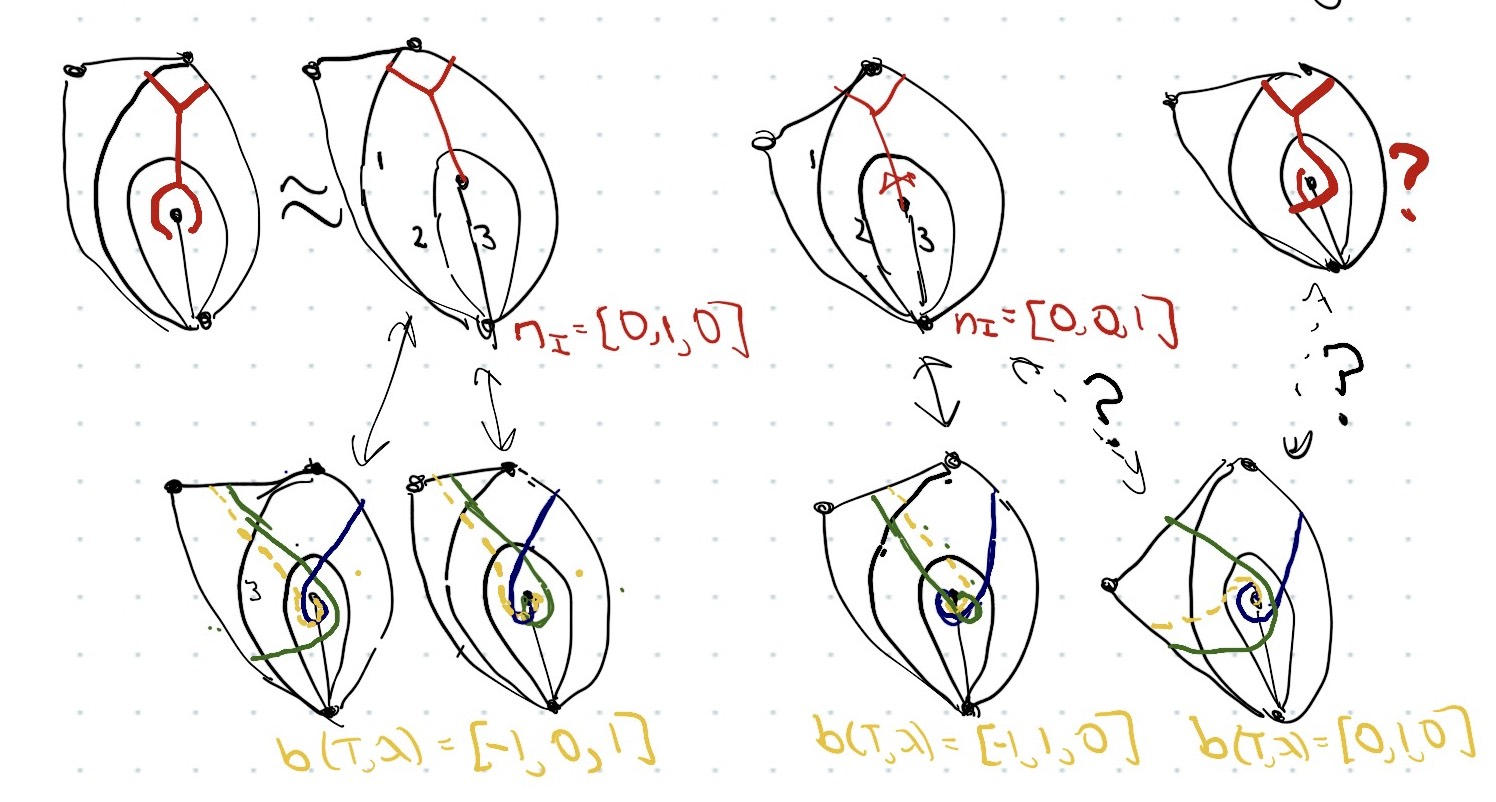
\includegraphics[scale=.2]{new_ibeam.jpg}
\end{remark}

\begin{figure}
\caption{Some simple examples}
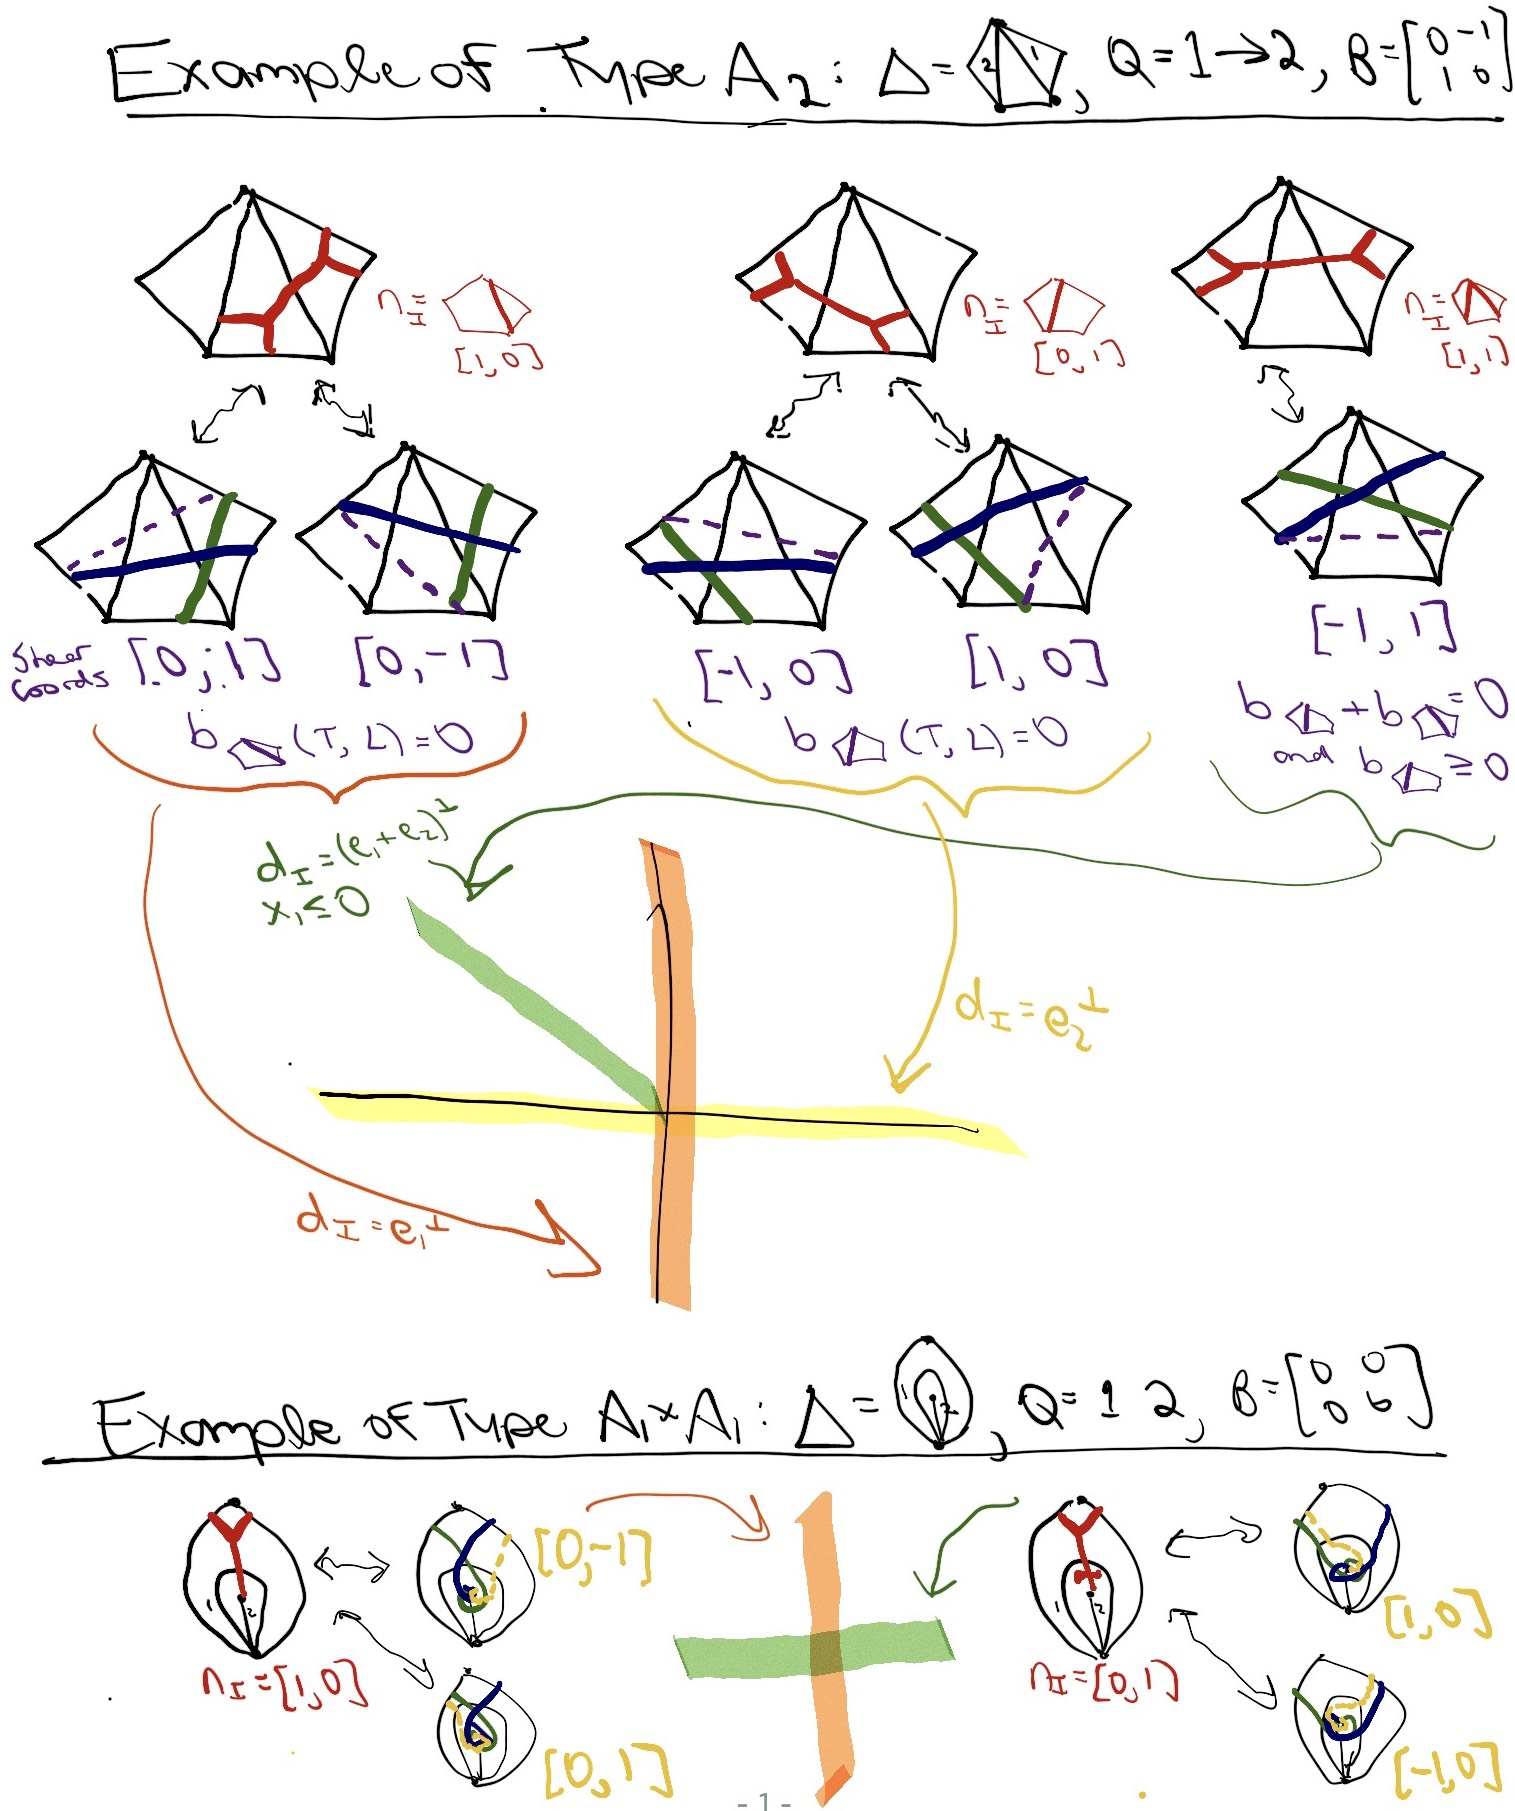
\includegraphics[scale=.25]{ibeam_examples.jpg}
\end{figure}


\newpage

\section{A possible alternative to I-beams and joints}

\begin{definition}
Given a triangulation $\Delta$ of unpunctured\margin[GM]{I haven't attempted punctured surfaces yet.} $(\S,\M)$, a \newword{barricade} $B$ in $\Delta$ is given by a topological graph embedded in $\S$, such that, when restricted to the neighborhood of a triangle in $\Delta$, the connected components are isotopic to one of the pictures in Figure \ref{fig: local barricade}.
%\begin{itemize}
%	\item each degree $1$ vertex lie in the interiors of arcs of $\Delta$ (or in punctures), and
%	\item each degree $3$ vertex lies in the interior of a triangle and the adjacent edges 
%\end{itemize}
\end{definition}

\begin{figure}[h!t]
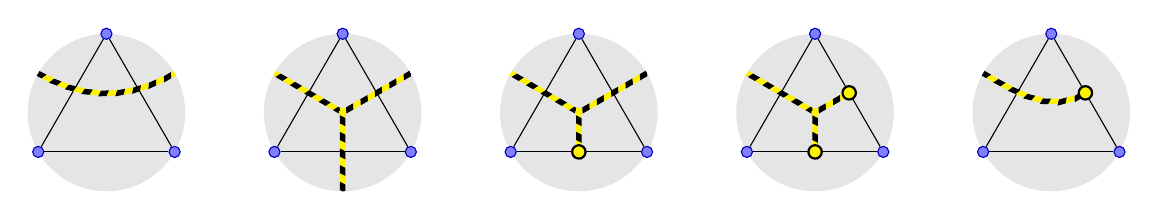
\begin{tikzpicture}[scale=1]
\begin{scope}[xshift=0cm]
	\path[fill=black!10] (0,0) circle (1);
	\node[marked] (1) at (90:1) {};
	\node[marked] (2) at (-30:1) {};
	\node[marked] (3) at (210:1) {};
	\draw (1) to node[below] {} (2);
	\draw (2) to node[below] {} (3);
	\draw (3) to node[below] {} (1);
	\clip (0,0) circle (1);
	\draw[barricade,out=210,in=-30] (30:1) to (150:1);
\end{scope}
\begin{scope}[xshift=3cm]
	\path[fill=black!10] (0,0) circle (1);
	\node[marked] (1) at (90:1) {};
	\node[marked] (2) at (-30:1) {};
	\node[marked] (3) at (210:1) {};
	\draw (1) to node[below] {} (2);
	\draw (2) to node[below] {} (3);
	\draw (3) to node[below] {} (1);
	\clip (0,0) circle (1);
	\draw[barricade] (150:1) to (0,0);
	\draw[barricade] (0,0) to (30:1);
	\draw[barricade] (0,0) to (270:1);
\end{scope}
\begin{scope}[xshift=6cm]
	\path[fill=black!10] (0,0) circle (1);
	\node[marked] (1) at (90:1) {};
	\node[marked] (2) at (-30:1) {};
	\node[marked] (3) at (210:1) {};
	\draw (1) to node[below] {} (2);
	\draw (2) to node[below] {} (3);
	\draw (3) to node[below] {} (1);
	\clip (0,0) circle (1);
	\draw[barricade] (150:1) to (0,0);
	\draw[barricade] (0,0) to (30:1);
	\draw[barricade] (0,0) to (270:.5);
	\node[barricade vertex] (b) at (270:.5) {};
\end{scope}
\begin{scope}[xshift=9cm]
	\path[fill=black!10] (0,0) circle (1);
	\node[marked] (1) at (90:1) {};
	\node[marked] (2) at (-30:1) {};
	\node[marked] (3) at (210:1) {};
	\draw (1) to node[below] {} (2);
	\draw (2) to node[below] {} (3);
	\draw (3) to node[below] {} (1);
	\clip (0,0) circle (1);
	\draw[barricade] (150:1) to (0,0);
	\draw[barricade] (0,0) to (30:.5);
	\draw[barricade] (0,0) to (270:.5);
	\node[barricade vertex] (a) at (30:.5) {};
	\node[barricade vertex] (b) at (270:.5) {};
\end{scope}
\begin{scope}[xshift=12cm]
	\path[fill=black!10] (0,0) circle (1);
	\node[marked] (1) at (90:1) {};
	\node[marked] (2) at (-30:1) {};
	\node[marked] (3) at (210:1) {};
	\draw (1) to node[below] {} (2);
	\draw (2) to node[below] {} (3);
	\draw (3) to node[below] {} (1);
	\clip (0,0) circle (1);
	\draw[barricade,out=210,in=-30] (30:.5) to (150:1);
	\node[barricade vertex] (a) at (30:.5) {};
\end{scope}
\end{tikzpicture}
\caption{Local pictures of barricades (up to rotation and reflection)}
\label{fig: local barricade}
\end{figure}

A \newword{short leaf}\margin[GM]{I can't decide if we want to allow non-short leaves in the definition. They make the proof of Prop. \ref{prop: inequalities} easier, but they don't appear in barricades related to the scattering diagram.} is a leaf whose adjacent vertex is in the adjacent triangle (e.g. the third and fourth local picture in Figure 
\ref{fig: local barricade}). A \newword{long leaf} is a leaf on the boundary of $\S$. \marginN{The definition of long leaf doesn't seem to be used.}

Barricades are considered up to isotopy within the set of barricades (so leaves must remain on arcs in $\Delta$). 
A measured lamination $\mu$ is \newword{compatible} with a barricade $B$ if there is are equivalent $\mu'$ and $B'$ such that $\mu'$ intersects $\Delta$ minimally and $\mu'$ and $B'$ do not intersect.%\margin[GM]{`Compatible' is a bit fiddly to define, since we need to be able to move the barricade around, but not 

\begin{prop}\label{prop: inequalities}
Given a barricade $B$, a measured lamination $\mu$ is compatible with $B$ iff the following inequalities hold.
\begin{itemize}
	\item For each path in $B$ which begins with a right turn and ends with a left turn,
	\[ S_{1}(\mu) + S_{2}(\mu) + ... + S_{n}(\mu) \geq 0\]
	where $S_1, S_2,...,S_n$ are the shear coordinates of the arcs in $\Delta$ crossed by $P$.
	\item For each path in $B$ which begins with a left turn and ends with a right turn, 
	\[ S_{1}(\mu) + S_{2}(\mu) + ... + S_{n}(\mu) \leq 0\]
	where $S_1, S_2,...,S_n$ are the shear coordinates of the arcs in $\Delta$ crossed by $P$.
	\item For each cycle in $B$, 
	\[ S_{1}(\mu) + S_{2}(\mu) + ... + S_{n}(\mu) = 0\]
	where $S_1, S_2,...,S_n$ are the shear coordinates of the arcs in $\Delta$ crossed by $P$.
\end{itemize}
\end{prop}

%Given a barricade $B$, let $C_B\subset \mathbb{R}^\Delta$ be the set of measured laminations which are compatible with $B$.

\begin{corollary}
Given a barricade $B$, the set $C_B\subset \mathbb{R}^\Delta$ of measured laminations which are compatible with $B$ is a closed cone. 
\end{corollary}



%\begin{definition}
%Given an (ordinary, untagged) triangulation $\Delta$ of $(\S,\M)$, an \newword{I-beam} is a graph $I$ embedded in $\S$, such that, when restricted to the neighborhood of a triangle in $\Delta$, the connected components are isotopic to one of pictures in Figure \ref{fig: local I-beams}.
%\end{definition}

%\begin{figure}[h!t]
%\begin{tikzpicture}[scale=1]
%\begin{scope}[xshift=0cm]
%	\draw[fill=black!10, dashed] (0,0) circle (1);
%	\node[marked] (1) at (90:1) {};
%	\node[marked] (2) at (-30:1) {};
%	\node[marked] (3) at (210:1) {};
%	\draw (1) to node[below] {} (2);
%	\draw (2) to node[below] {} (3);
%	\draw (3) to node[below] {} (1);
%	\draw[red,out=210,in=-30] (30:1) to (150:1);
%\end{scope}
%\begin{scope}[xshift=3cm]
%	\draw[fill=black!10, dashed] (0,0) circle (1);
%	\node[marked] (1) at (90:1) {};
%	\node[marked] (2) at (-30:1) {};
%	\node[marked] (3) at (210:1) {};
%	\draw (1) to node[below] {} (2);
%	\draw (2) to node[below] {} (3);
%	\draw (3) to node[below] {} (1);
%	\node[inner sep=0.5mm,circle,draw=red] (a) at (30:.5) {};
%	\node[inner sep=0.5mm,circle,draw=red] (b) at (270:.5) {};
%	\draw[red] (150:1) to (0,0);
%	\draw[red] (0,0) to (a);
%	\draw[red] (0,0) to (b);
%\end{scope}
%%\begin{scope}[xshift=6cm]
%%	\draw[fill=black!10, dashed] (0,0) circle (1);
%%	\node[marked] (1) at (90:1) {};
%%	\node[marked] (2) at (270:1) {};
%%	\node[marked] (3) at (0,0) {};
%%	\draw[out=-15,in=15] (1) to (2);
%%	\draw[out=195,in=165] (1) to (2);
%%	\draw[out=-60,in=60] (1) to (3);
%%	\draw[out=-120,in=120] (1) to (3);
%%	\draw[red] (3) to (0,-.5);
%%	\draw[red,out=-30,in=210] (0,.-.5) to (0:1);
%%	\draw[red,out=210,in=-30] (0,.-.5) to (180:1);
%%\end{scope}
%%\begin{scope}[xshift=9cm]
%%	\draw[fill=black!10, dashed] (0,0) circle (1);
%%	\node[marked] (1) at (90:1) {};
%%	\node[marked] (2) at (270:1) {};
%%	\node[marked] (3) at (0,0) {};
%%	\draw[out=-15,in=15] (1) to (2);
%%	\draw[out=195,in=165] (1) to (2);
%%	\draw[out=-60,in=60] (1) to (3);
%%	\draw[out=-120,in=120] (1) to (3);
%%	\draw[red] (3) to (0,-.5);
%%	\draw[red,out=-30,in=210] (0,.-.5) to (0:1);
%%	\draw[red,out=210,in=-30] (0,.-.5) to (180:1);
%%\end{scope}
%\end{tikzpicture}
%\caption{Local pictures of I-beams (no punctures)}
%\label{fig: local I-beams}
%\end{figure}



%\begin{thm}
%The scattering diagram of $(\S,\M)$ in $\mathbb{R}^\Delta$ has a wall for each minimal barricade of codimension $1$ (supported on the compatible cone), and a joint for each minimal barricade of codimension $2$ (supported on the compatible cone).
%\end{thm}

%\begin{ex}
%
%Consider the following barricade.
%
%\begin{center}
%\begin{tikzpicture}
%\begin{scope}[scale=.5]
%	\draw[fill=black!10] (0,0) circle (2);
%	\node[marked] (1) at (90:2) {};
%	\node[marked] (2) at (18:2) {};
%	\node[marked] (3) at (306:2) {};
%	\node[marked] (4) at (234:2) {};
%	\node[marked] (5) at (162:2) {};	
%%	\draw (1) to (2);
%%	\draw (2) to (3);
%%	\draw (3) to (4);
%%	\draw (4) to (5);
%%	\draw (5) to (1);
%	\draw (1) to (3);
%	\draw (1) to (4);
%	\draw[barricade] (54:2) to (-78:2);
%	
%\end{scope}
%\end{tikzpicture}
%\end{center}
%
%\end{ex}

%\newpage

\section{Proof of Proposition \ref{prop: inequalities}}

Let us collectively refer to the inequalities in Proposition \ref{prop: inequalities} as the \newword{compatibility inequalities} for $B$ and $\mu$. 

A barricade is \newword{simple} if it is connected and has no degree $3$ vertices. We start by proving a stronger version of Proposition \ref{prop: inequalities} in the case of a simple barricades.

\begin{lemma}\label{lemma: simplebarricade}
Let $B$ be a simple barricade in $\Delta$. A measured lamination $\mu$ is compatible with $B$ iff it satisfies the compatibility inequalities.
\end{lemma}

\begin{proof}[Proof idea]
Induction, I hope. I don't know about loops, though.
\end{proof}
	
\begin{lemma}\label{lemma: simplesub}
A measured lamination $\mu$ is compatible with a barricade $B$ iff $\mu$ is compatible with every simple sub-barricade of $B$.
\end{lemma}

\begin{proof}[Proof idea]
If they are incompatible, there should be some unmarked curve that is crossed.
\end{proof}

\begin{proof}[Proof of Proposition \ref{prop: inequalities}]
Assume $\mu$ is compatible with $B$. For any path or cycle in $B$, there is a simple sub-barricade $B'$ containing that path or cycle which is also compatible with $\mu$, and so the associated compatibility inequality holds by Lemma \ref{lemma: simplebarricade}.

Assume the compatibility inequalities hold for $\mu$ and $B$. Then they also hold for any simple sub-barricade of $B$, and so by Lemma \ref{lemma: simplebarricade} $\mu$ is compatible with each of them. By Lemma \ref{lemma: simplesub}, $\mu$ is compatible with $B$.
\end{proof}

\section{Minimal barricades}

%\begin{prop}
%If a measured lamination $\mu$ is compatible with a barricade $B$, 
%\end{prop}

\begin{definition}
The \newword{codimension} of a barricade is the codimension of (the span of) the compatible cone. A barricade is \newword{minimal} if it has no sub-barricades of the same codimension.
\end{definition}

Easy observation: all leaves in a minimal barricade are short, since they can be cut off without increasing the codimension.

%If $B$ has no loops, the span of the compatible cone has codimension equal to the number of edges in $B$ whose endpoints are degree $3$ vertices.



\begin{conj}
The codimension of a barricade $B$ is 
\[ (\text{$\#$ of edges between trivalent vertices}) + (\text{$\#$ of loops without leaves}) \]
\end{conj}

\begin{corollary}
The minimal barricades of codimension $1$ are:
\begin{itemize}
	\item Trees with $4$ leaves, all short.
	%which are locally isomorphic to the pictures in Figure \ref{fig: local I-beams}.
	\item A cycle with $0$ leaves.
\end{itemize}
\end{corollary}

\begin{corollary}
The minimal barricades of codimension $2$ are:
\begin{itemize}
	\item Trees with $5$ leaves, all short.
	\item A cycle with $2$ leaves, all short.
	\item Disjoint unions of $2$ minimal barricades of codimension $1$.
\end{itemize}
\end{corollary}

\begin{lemma}
If $B$ and $B'$ are minimal barricades, then 
\[ C_B\cap C_{B'} = \bigcup _i C_{B_i} \]
where each of the $B_i$ are minimal barricades. 
\end{lemma}

%\begin{conj}
%The codimension of a barricade $B$ is 
%\begin{align*}
%&\frac{3(\text{$\#$ of branches}) - \text{$\#$ of leaves}}{2} + (\text{$\#$ of components without branches})
%%\#&\text{ of edges in $B$ with a branch at each endpoint} \\
%%&+ \#\text{ of loops (i.e. cycles without branches)} \\
%%&+ \text{total genus of components of $\S\smallsetminus B$ that don't contain marked points}\\
%\end{align*}
%\end{conj}

\section{The scattering diagram of $(\S,\M)$}

We fix a triangulation $\Delta$ of $(\S,\M)$, and we use the language of barricades to construct a scattering diagram in $\mathbb{R}^\Delta$. We distinguish two kinds of minimal barricades of codimension $1$.
Construct a scattering diagram $\mathfrak{D}$ in $\mathbb{R}^\Delta$ as follows.
\begin{itemize}
	\item A \newword{I-beam} is a tree with $4$ short leaves. For each {I-beam} $B$, $\mathfrak{D}$ has a wall
	\[ (C_B, 1+x^{\mathsf{B}n} )\]
	where $n\in\mathbb{N}^\Delta$ counts the transverse crossings of $B$ and the arcs in $\Delta$.
	\item A \newword{non-shielding loop} is a cycle with $0$ leaves, such that each component of the complement contains a marked point. For each {non-shielding loop} $B$, $\mathfrak{D}$ has a wall
	\[ \left(C_B, (1-x^{\mathsf{B}n})^{-2} \right)\]
	where $n\in\mathbb{N}^\Delta$ counts the transverse crossings of $B$ and the arcs in $\Delta$.
\end{itemize}

\begin{theorem}\label{thm: consistent}
The scattering diagram $\mathfrak{D}$ is consistent, and is the GHKK scattering diagram of the seed $\Delta$ in the cluster algebra associated to $(\S,\M)$.
\end{theorem}

\subsection{Proof of Theorem \ref{thm: consistent}}

\begin{lemma}
The joints of $\mathfrak{D}$ are as follows.%are $C_B$, as $B$ runs over the minimal barricades of codimension $2$.
\begin{itemize}
	\item If $B$ is a tree with 5 short leaves, then $C_B$ is a joint which is contained in the 3 walls; specifically, the 3 I-beams contained in $B$.
	\item If $B$ is a cycle with 2 short leaves on the same side, then $C_B$ is a joint which is contained in 2 or 3 walls; specifically, the 2 I-beams contained in $B$, and the cycle (if it is non-shielding).
	\item If $B$ is a cycle with 2 short leaves on different sides, then $C_B$ is a joint which is contained in infinitely many walls; specifically, the infinitely-many I-beams contained in $B$, and the cycle.\footnote{Note that the cycle in this case must be non-shielding.}
	\item If $B$ is a disjoint union of $2$ I-beams or non-shielding loops, then $C_B$ is a joint contained in 2 walls.
\end{itemize}
\end{lemma}

\begin{thebibliography}{27}

\bibitem{cats1}
S. Fomin, M. Shapiro, and D. Thurston,
\textit{Cluster algebras and triangulated surfaces. I. Cluster complexes.}
Acta Math. \textbf{201} (2008), no. 1, 83--146. 

\bibitem{cats2}
S. Fomin and D. Thurston,
\textit{Cluster algebras and triangulated surfaces. Part II: Lambda lengths.}
Preprint, 2008.
(arXiv:1210.5569)

\bibitem{ca4}
S. Fomin and A. Zelevinsky,
\textit{Cluster Algebras IV: Coefficients.}
Compositio Mathematica \textbf{143} (2007), 112--164.

\bibitem{GHK}
M. Gross, P. Hacking, and S. Keel,
\textit{Birational geometry of cluster algebras.}
Algebraic Geometry \textbf{2} (2015) 137--175.

\bibitem{GHKK}
M. Gross, P. Hacking, S. Keel, and M. Kontsevich,
\textit{Canonical bases for cluster algebras.}
Preprint, 2014. \texttt{arXiv:1411.1394}

\bibitem{unisurface}
N. Reading,
\textit{Universal geometric cluster algebras from surfaces. }
Trans. Amer. Math. Soc. \textbf{366} no. 12 (2014), 6647--6685.

\bibitem{scatfan}
N. Reading, 
\textit{Scattering fans}. 
In preparation.

\bibitem{dominance}
N. Reading, 
\textit{Dominance phenomena: Mutation, scattering and cluster algebras}. 
In preparation.

\end{thebibliography}


\end{document}  